\documentclass{article}
\usepackage{amsmath}
\usepackage{hyperref}
\usepackage{graphicx}
\begin{document}
\begin{titlepage}
\title{EE 239AS \\Special Topics in Signals and Systems\\Project 1\\Regression Analysis\\Winter 2016} 
\author{Liqiang YU, Kaiming WANG and Jun FENG\\
904592975, 504592374, 304588434} 
\date{01-31-2016}
\end{titlepage}

\maketitle
\newpage
\tableofcontents
\newpage
\section{Introduction}
In this report, we implemented some regression models to fit the data within two datasets, including the linear regression, random forest regression, neural network regression and polynomial regression. We made some comparisons between the prediction results of different models based on root mean squared error(RMSE) and the coefficient of determination($R^2$).
Based on the statistics provided by models, we analyzed the significance of different features. In order to avoid overfitting, which often happens in the regression fitting problem, we implemented both cross-validation and regularization techniques. Moreover, since some of the features have no numerical meaning, we formatted them into binary features, which increase the number of features. \\
\\
The report is organized as follows : In section 2, we preprocessed the data and plotted the data to find some pattern. In section 3, The dataset was from a simulated traffic data on the backup system in a network system. We implemented both the linear regression model and random forest regression model to predict the copy size of the backup file and made some analysis and comparisons of the predictions. In section 4, we implemented the neural network model and polynomial regression model to fit the data and analyzed the impact of different parameters to the results. In section 5, we implement the piecewise linear regression and polynomial regressions. In section 6, we implement all the previous regression on the Boston Housing Dataset. In section 7, we introduce ridge and lasso regression techniques on this Dataset 
\section{Data Preprocessing}
\subsection{Feature Binarization}
After checking the data, there are seven features in the dataset named network\_ backup\_ dataset, including week, day of the week, backup start time, work flow ID, file name, size of backup and backup time. The target value is the size of backup, others are features. Therefore, first of all we need to transform non-numerical values into numerical values. However, consider "the day of the week" feature, "Tuesday" is not larger than "Monday", but "2" is larger than "1". So we need to make such kind of features into binary format. For instance, for "day of the week", we need to expand it into seven features, where it is 1 on the specified day and all the others 0. Finally, we have 64 features in total.
\subsection{Pattern Detection}
In order the find the pattern, we plot the figure of the copy size over time. The independent variable is the "Start Time - Hour of Day", the dependent variable is the copy size. There are six sampling times in a day and 20 days as a period. So the x axis is from 1 to 120. The figure is shown in figure \ref{fig:start_time}.
\begin{figure}[htbp]
\centering
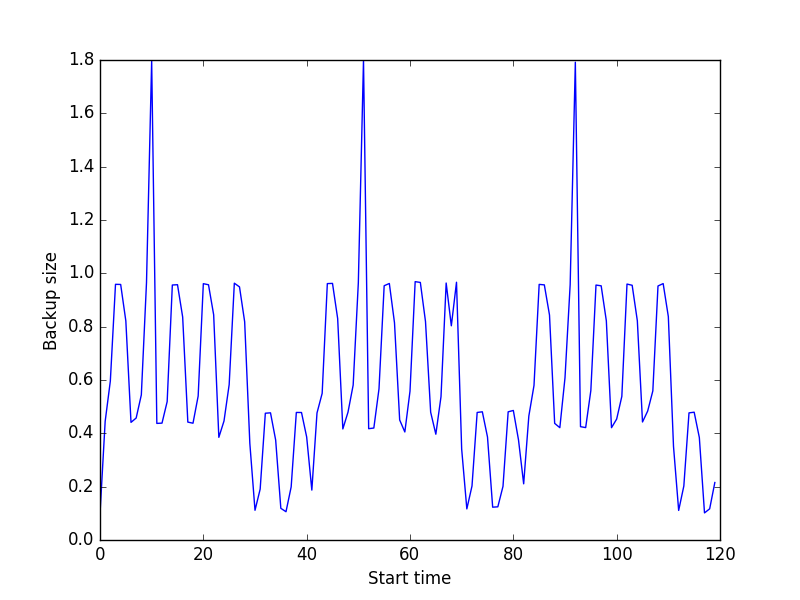
\includegraphics[width=.6\textwidth]{pattern_start.png}
\caption{The copy size of backup over start time}
\label{fig:start_time}
\end{figure}
From \ref{fig:start_time} we can see there is clearly a cycle between copy size and time. So we plot the copy size over days to find the cycle period. The result is shown in figure \ref{fig:day}. Hence we can predict that the cycle period is approximately a week.
\begin{figure}[htbp]
\centering
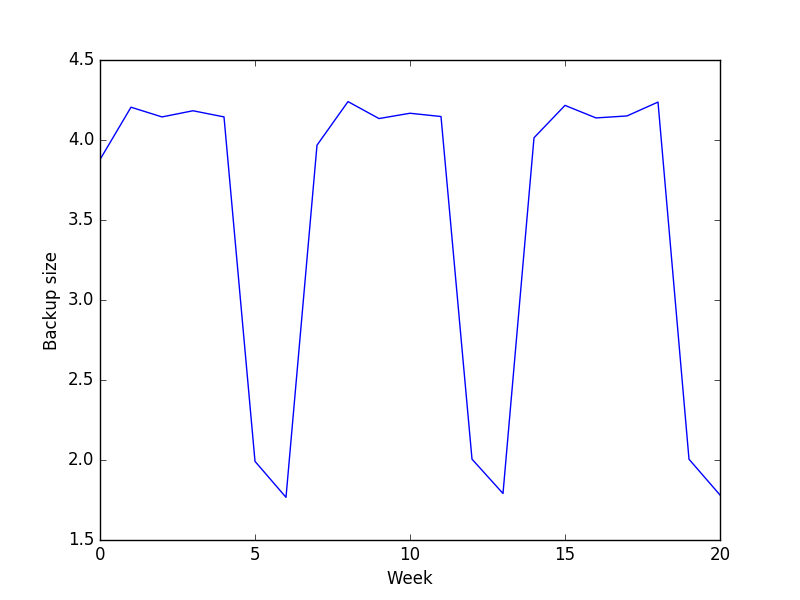
\includegraphics[width=.6\textwidth]{pattern_week.png}
\caption{The copy size of backup over week}
\label{fig:day}
\end{figure}
\section{Linear and Random Forest Regression}
\subsection{Linear Regression}
In the Linear Regression Model, we choose the copy size as the target variable and the other attributes as the features, the fit model is as follow
\begin{equation*}
\bar{Y} = X\alpha
\end{equation*}
where $\bar{Y}$ represents the target, $X$ represents the features vector and $\alpha$ is the linear coefficient. We used least square as the penalty function, which is
\begin{equation*}
min || Y - \bar{Y} ||_2
\end{equation*}
In order to avoid the overfitting problem, we implemented 10-fold cross-validation technique. First do a random shuffling over the data, then split them into 10 folds. Each time choose 9 of 10 as the train set and the other 1 fold as the test set. The Root Square Mean Error (RMSE) is shown in figure \ref{fig:rmse_lr}. The average RMSE is 0.071.
\begin{figure}[htbp]
\centering
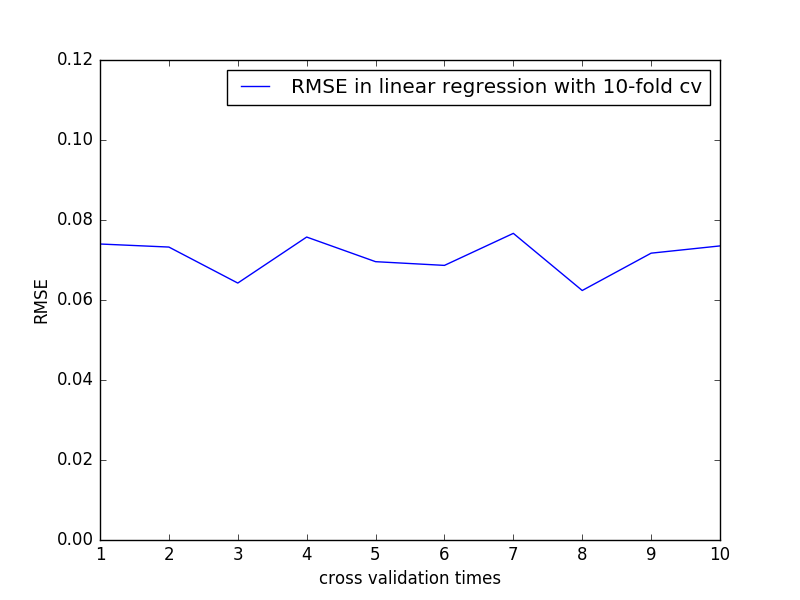
\includegraphics[width=.6\textwidth]{rmse_linear.png}
\caption{The copy size of backup over week}
\label{fig:rmse_lr}
\end{figure}
To evaluate the fitting accuracy of our model, “Fitted values VS actual values” and “residuals vs fitted values” are plotted. From figure \ref{fig:actual_pred}, we can see that most predicted values are close to the actual values. From figure \ref{fig:residual}, we can see that the residuals are distributed randomly around zero axis, which means the model is proper.\\
\begin{figure}[htbp]
\centering
\begin{minipage}[t]{0.45\textwidth}
\centering
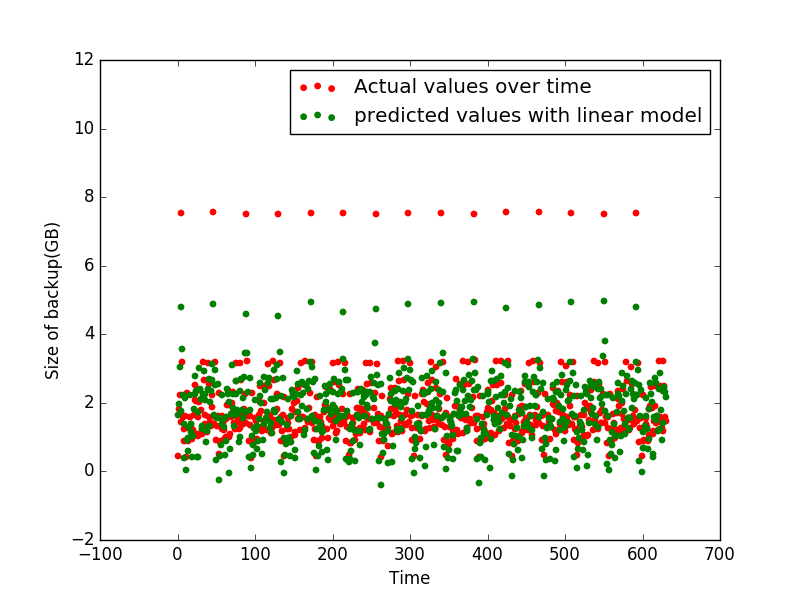
\includegraphics[width=\textwidth]{actual_pred.png}
\caption{Actual VS predicted}
\label{fig:actual_pred}
\end{minipage}
\begin{minipage}[t]{0.45\textwidth}
\centering
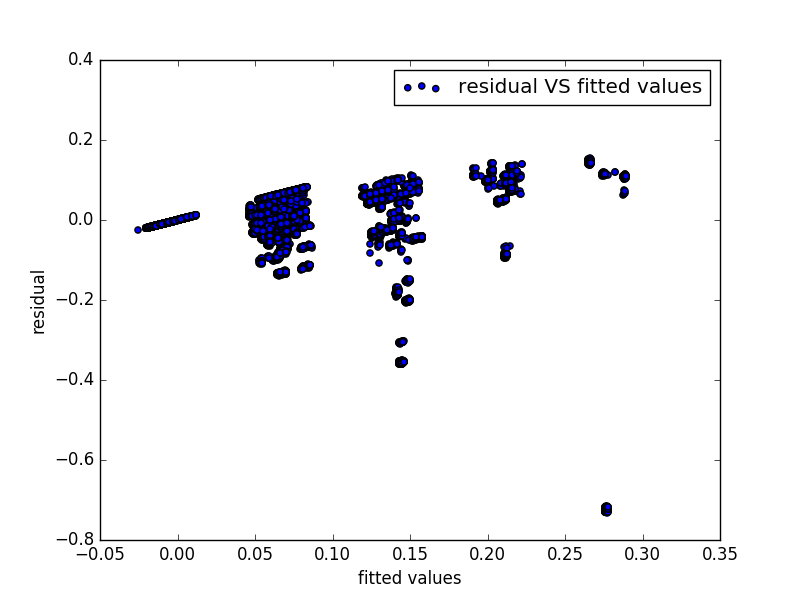
\includegraphics[width=\textwidth]{residual.png}
\caption{Residual VS fitted values}
\end{minipage}
\label{fig:residual}
\end{figure}
\\
As for the significance of different variables, we choose p-value as the evaluation criterion. The p-value of the six features is shown in figure \ref{fig:p6}.\\
\begin{figure}[htbp]
\centering
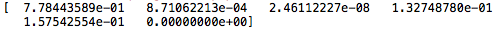
\includegraphics[width=.8\textwidth]{pvalue-6.png}
\caption{p-value of 6 features}
\label{fig:p6}
\end{figure}
\\
Therefore the most important two features are "Backup start time - Hour of the day" and "Backup Time" because their p-values are close to 0.
For 64 features, the p-value matrix is shown below.\\
\begin{figure}[htbp]
\centering
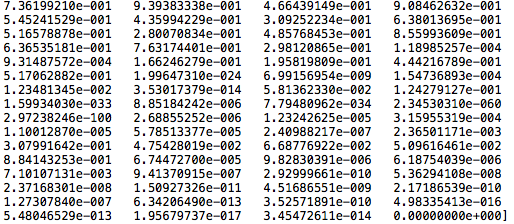
\includegraphics[width=.8\textwidth]{pvalue-64.png}
\caption{p-value of 64 features}
\label{fig:p64}
\end{figure}
\subsection{Random Forest Regression}
For random forest regression, we initialize the model with parameters : number of trees 20, depth of trees 4, max features 64. The average RMSE is 0.0297. After tuning the parameters, we have the best RMSE 0.00943. The parameters are : number of trees 32, depth of trees 12, max features 64. The best RMSE is shown in figure \ref{fig:rf}.\\
\begin{figure}[htbp]
\centering
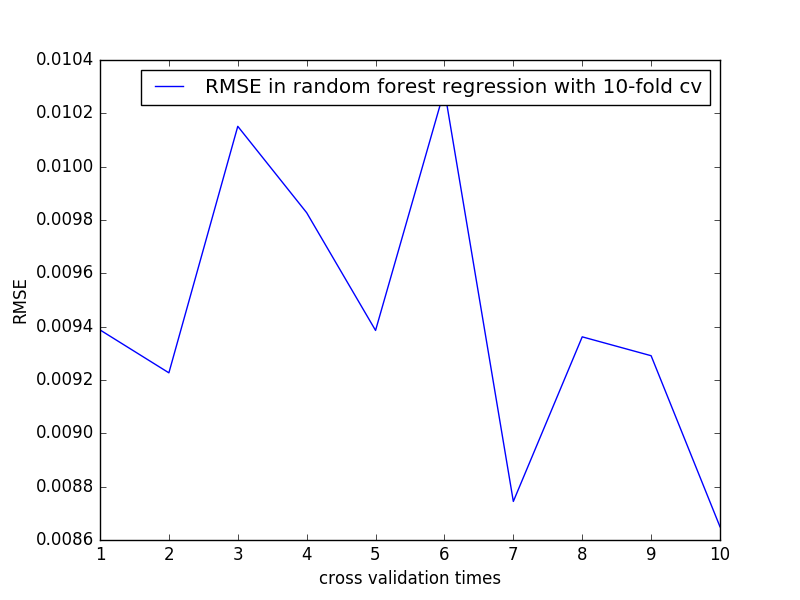
\includegraphics[width=.6\textwidth]{rf_rmse.png}
\caption{The best RMSE of random forest regression}
\label{fig:rf}
\end{figure}
\subsection{The comparison between two models}
The comparison between Linear Regression and Random Forest Regression is shown in figure \ref{fig:comp}. Random forest is a lot better than linear regression.\\
\begin{figure}[htbp]
\centering
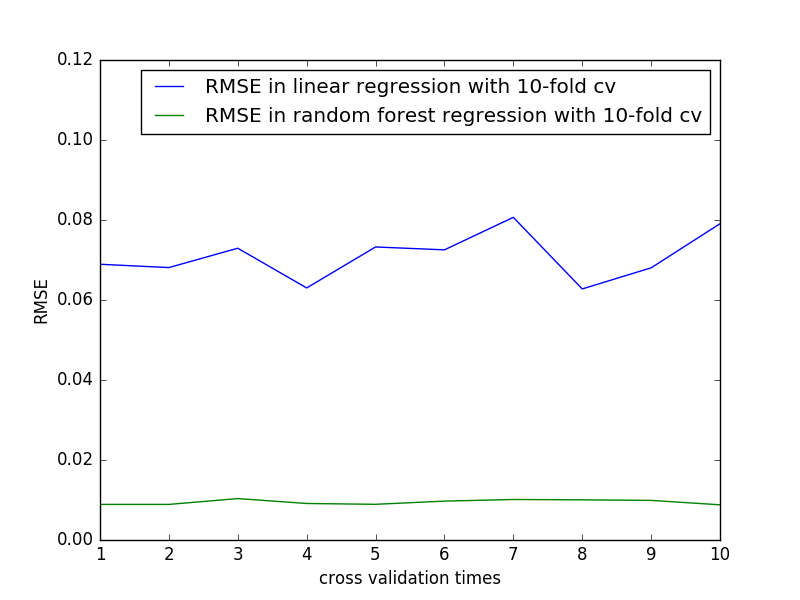
\includegraphics[width=.6\textwidth]{compare.png}
\caption{The comparison between Linear and Random Forest Regression}
\label{fig:comp}
\end{figure}
\\
The prediction of the random forest model is shown in figure \ref{fig:r_pred}. We can see the cycle period is around 42 backup times, which is about a week, so the pattern is the same with the actual values.
\begin{figure}[htbp]
\centering
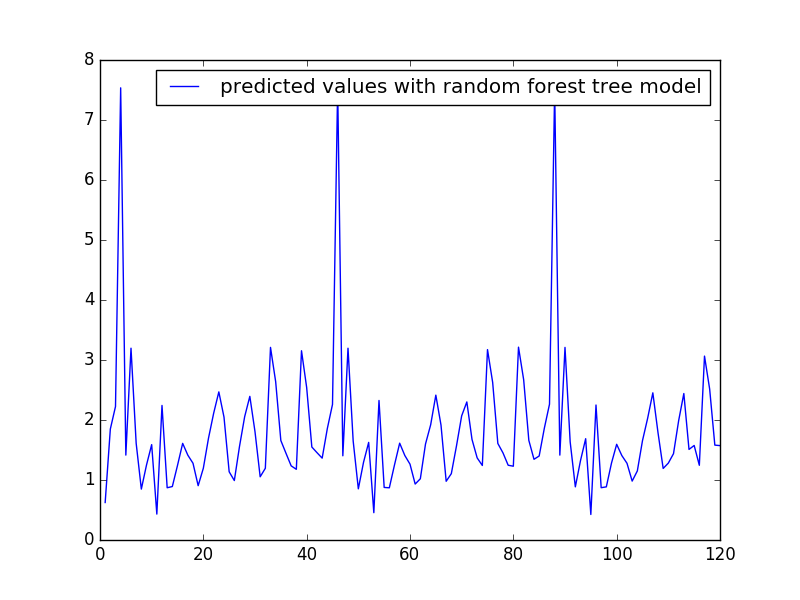
\includegraphics[width=.6\textwidth]{random_pred.png}
\caption{The prediction of the random forest}
\label{fig:r_pred}
\end{figure}
\section{Neural Network}
In the neural network model, we choose the feedforward network with the backpropagation trainer. The main parameters are the number of layers, the kind of hidden layers and the number of iteration before convergence. After lots of experience, we find that sigmoid layer is proper for hidden layers and linear layer is proper for the output layer. The optimal number of layers is 7. The RMSE reduces when the number of iteration is increasing, however it is too slow with large iteration number. So we set it to be 10. The best RMSE we can get is 0.0827. The RMSE is shown in figure \ref{fig:nn}.
\begin{figure}[htbp]
\centering
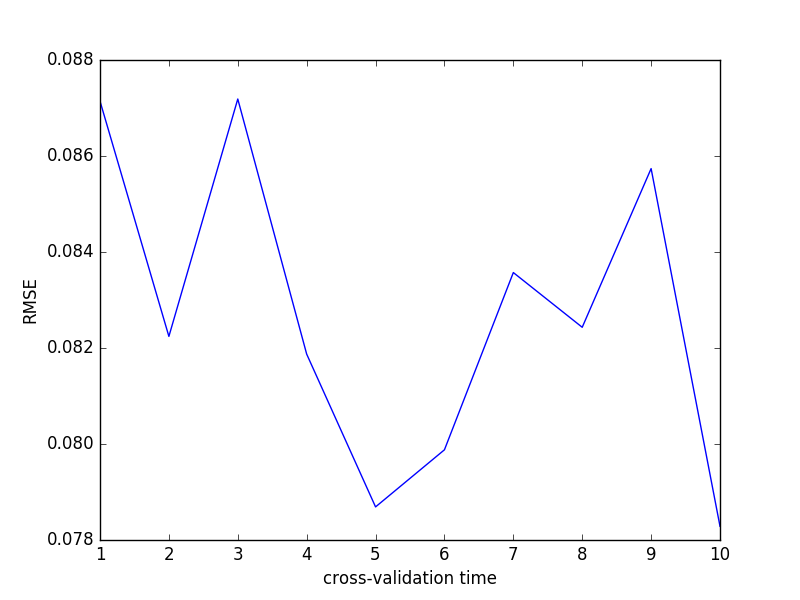
\includegraphics[width=.6\textwidth]{nn.png}
\caption{The RMSE of neural network model}
\label{fig:nn}
\end{figure}
\section{Piece-wise Linear Regression and Polynomial Regression}
\subsection{Piece-wise Linear Regression}
We just divide the all tuples according to their work-flow \#,  then implement the linear regression respectively which is illustrated by figure \ref{fig:wf}. However, we find that sometimes, piecewise regression does not necessarily benign the RMSE. It is consistent to the most cases: at most time, more data and more features can bring about a more reliable regression.
\begin{figure}[htbp]
\centering
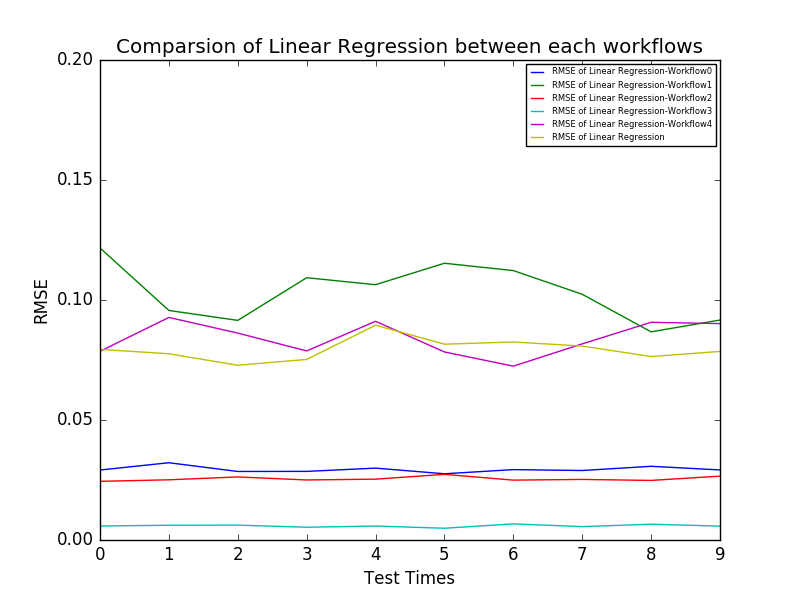
\includegraphics[width=.6\textwidth]{wf.png}
\caption{Piecewise Linear Regression}
\label{fig:wf}
\end{figure}
\subsection{Polynomial Regression}
By implying the PolynomialFeatures of Scikit-Learn, we can do polynomial regression. However, when the degree go higher and higher, overfitting may happened. Just as in figure \ref{fig:pr1}. According to the figure, the threshold of the degree is 5. Cross validation can help us to decide the degree of polynomial function.
\begin{figure}[htbp]
\centering
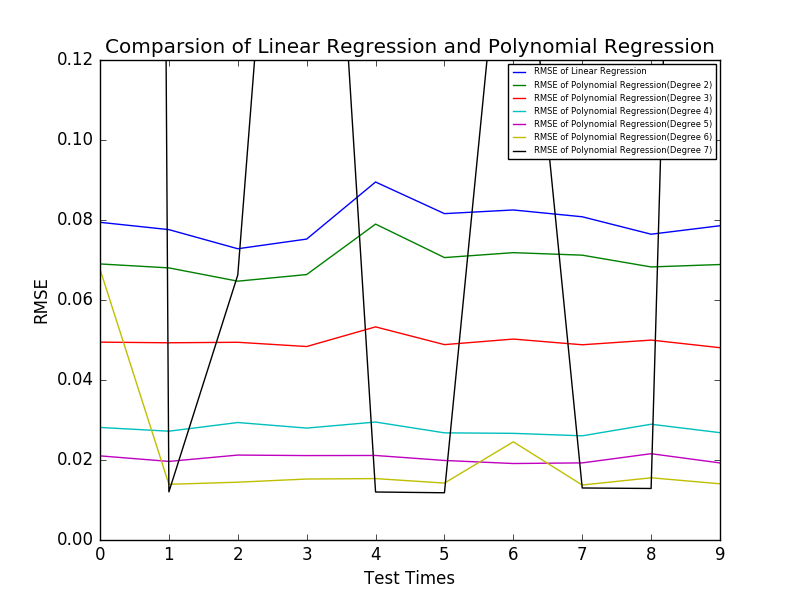
\includegraphics[width=.6\textwidth]{pr1.png}
\caption{Polynomial Regression}
\label{fig:pr1}
\end{figure}
\section{Linear and Polynomial Regression of Boston Datasets}
\subsection{Linear Regression}
Similar as the linear part of Chapter 3, we also implemented 10-fold cross validation here. And the RMSEs are shown in Figure \ref{fig:RMSEs}, and the mean of them is about 4.7403.
\begin{figure}[htbp]
\centering
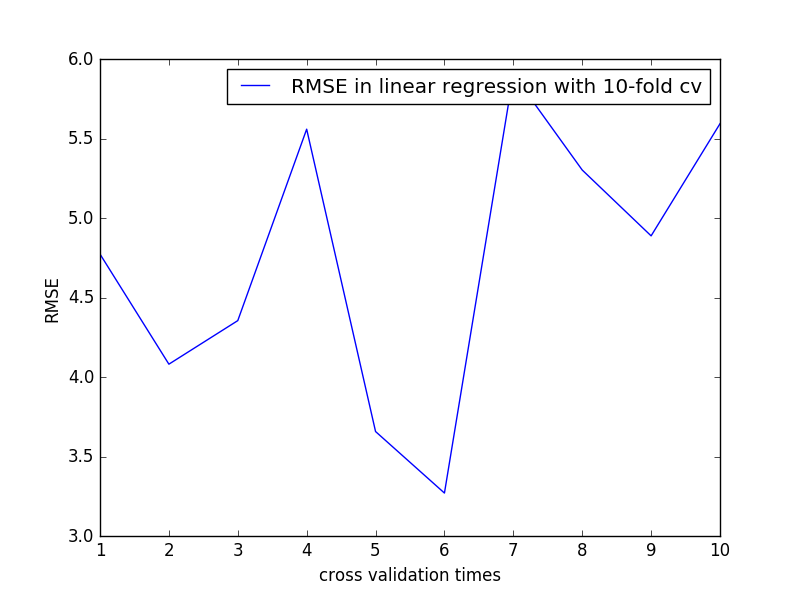
\includegraphics[width=.6\textwidth]{RMSEs.png}
\caption{Linear Regression of Boston}
\label{fig:RMSEs}
\end{figure}
To evaluate how well our model fit the data, we provide two graphs. The first one is shown as Figure \ref{fig:fitted_actual}, which is the scattered plot of actual and fitted MEDV values. And we can see that most of them overlaps. The other graph is the residuals versus fitted values, showed in Figure \ref{fig:residual_fitted}. Since most of them are clustered around 0 of y-axis, we are confirmed that our model fits the data quite well.
\begin{figure}[htbp]
\centering
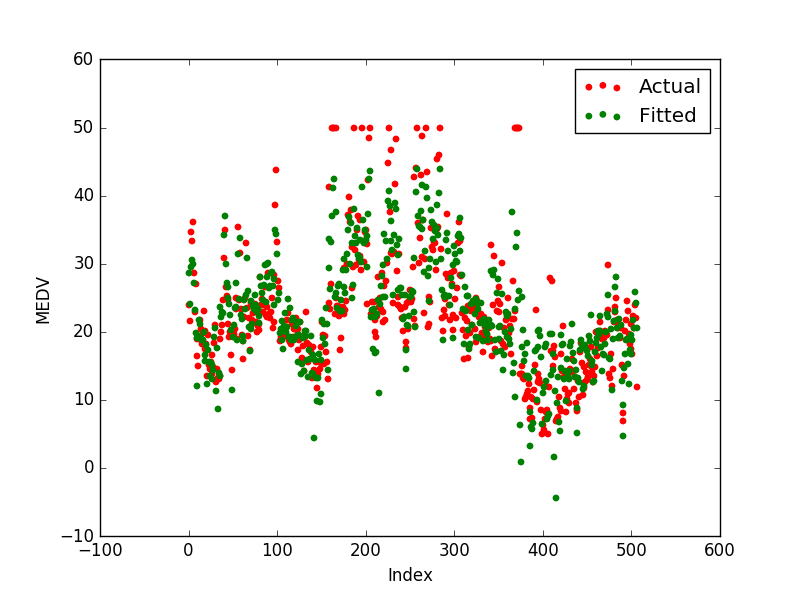
\includegraphics[width=.6\textwidth]{fitted_actual.png}
\caption{Scattered Plot of Actual and Fitted MEDV Values}
\label{fig:fitted_actual}
\end{figure}
\begin{figure}[htbp]
\centering
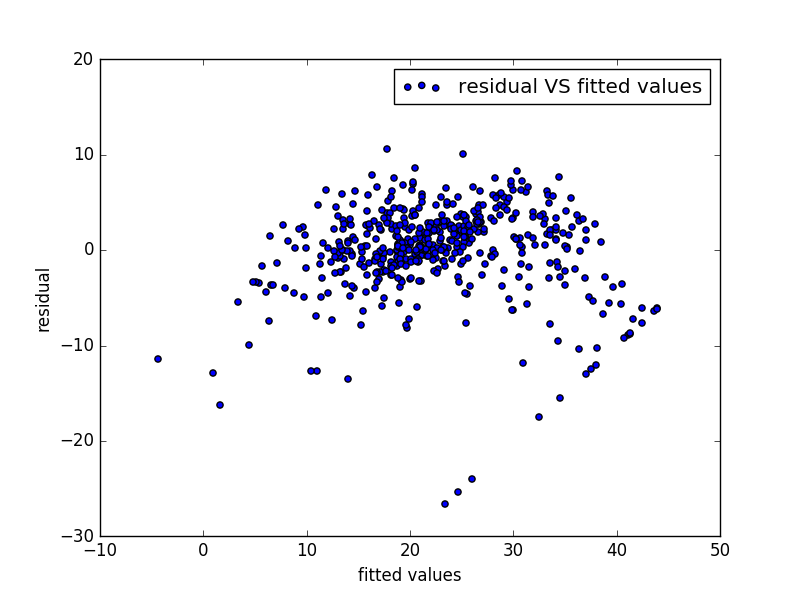
\includegraphics[width=.6\textwidth]{residual_fitted.png}
\caption{Residuals Versus Fitted Values}
\label{fig:residual_fitted}
\end{figure}
For the analyzation of significance of different features, we still use the p-value as before.  P-value of the 13 features are shown in Figure \ref{fig:feature13}, while those of 21 features are shown in Figure \ref{fig:feature21}. From them, we know that the three smallest p-values are the sixth, the third last and the last, which means that the corresponding features are the most significant ones. Particularly, they are the RM, PTRATIO and LSTAT. Later, when we were using the Lasso regression model and the α parameter is set as 0.1, we noticed that the only regression coefficients remain nonzero are exactly corresponding to those mentioned above, which means only the most important features are kept.
\begin{figure}[htbp]
\centering
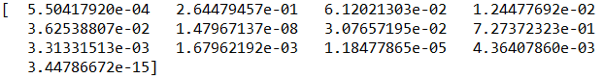
\includegraphics[width=.6\textwidth]{feature13.png}
\caption{P-value of the 13 Features}
\label{fig:feature13}
\end{figure}
\begin{figure}[htbp]
\centering
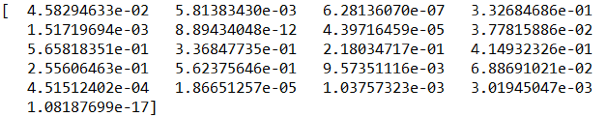
\includegraphics[width=.6\textwidth]{feature21.png}
\caption{P-value of the 21 Features}
\label{fig:feature21}
\end{figure}
\subsection{Polynomial Regression}
We do the same polynomial regression on target of Boston dataset, just like in part 3, this time the optimal degree of fit is just 2, which is illustrated in Figure \ref{fig:problem4-2}.
\begin{figure}[htbp]
\centering
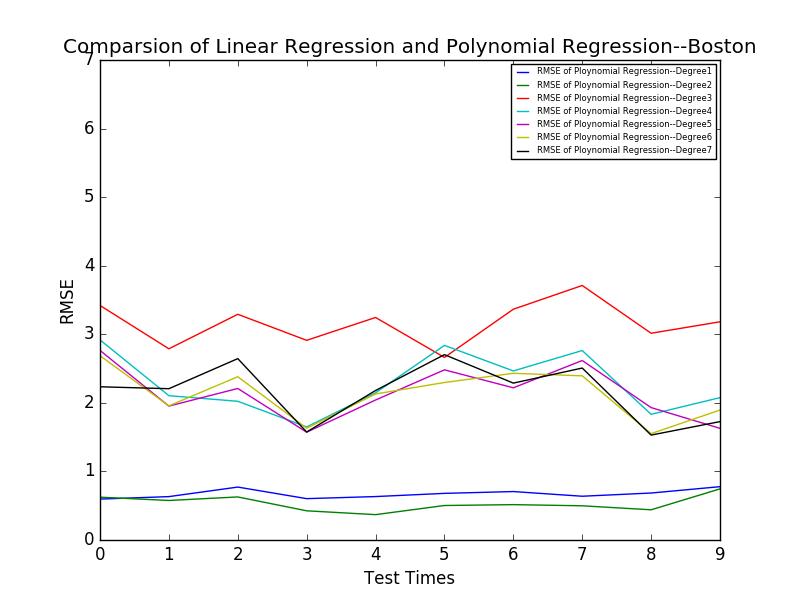
\includegraphics[width=.6\textwidth]{problem4-2.png}
\caption{Polynomial Regression}
\label{fig:problem4-2}
\end{figure}
\section{Lasso \& Ridge Regularization}
In machine learning, over fitting is likely to happens when a model is excessively complicated. Under this situation, the machine only memorizes the training data, instead of learning to predict the data from given features. In our problem, we have only about 500 tuple of data with 20 different features. Thus, the chance of our model to memorize data from these features is relatively high.
Before, we use cross validation to limit the affection of over fitting during the assessing of a model. In this way, we can only determine if a given model is good or not. Instead, if we want to generate better learning models with little over fitting, we may use method as regularization.
In regularization, we introduce a regularization term or so called loss function, which is usually a penalty on the complexity of our model. Therefore, it can improve the generalization ability of our model.
\subsection{Lasso Regularization}
In Lasso regularization, the regularization term is considering the -norm of the regression coefficient vector. And the penalty function has the following form:
\begin{equation*}
min\frac{1}{2n}||Y-X\beta||^2_2+\alpha||\beta||_1
\end{equation*}
For different extent of penalty on the complexity, we can choose various value of α. And in our solution, we choose it in the range ${0.1,0.01,0.001}$ as required. The corresponding performance of the regression model is shown in Figure \ref{fig:lar}, from which we can see that the RMSE is smaller with a little value of $\alpha$. 
\begin{figure}[htbp]
\centering
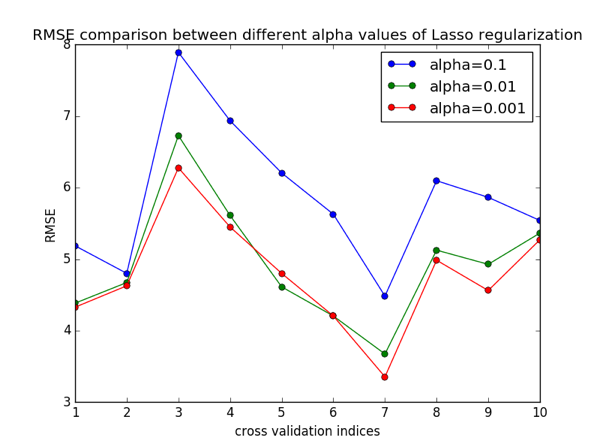
\includegraphics[width=.6\textwidth]{lar.png}
\caption{Lasso Regularization of Boston Dataset}
\label{fig:lar}
\end{figure}
After further research, we know that the result of linear regression almost overlaps the result of $\alpha=0.001$, which means that the RMSE of pure linear regression is smaller than those of Lasso regression. Thus, in this problem, the control of over fitting does not bring a better model to us. However, this does not mean it is useless. After checking the result of the regression coefficients, we are shocked by its sparsity. When $\alpha=0.1$, only 3 coefficients are nonzero and all the other 17 are 0. Thus, in this way, we have found a great sparse solution of our problem.
\subsection{Ridge Regularization}
In Ridge regularization, the regularization term is considering the $l_2$-norm of regression coefficient vector. And the penalty function has the following form:
\begin{equation*}
min\frac{1}{2n}||Y-X\beta||^2_2+\alpha||\beta||_1
\end{equation*}
Similar as Lasso regularization, we set the value of α in the range \{0.1,0.01,0.001\} and the performance of our regression models are shown in Figure  \ref{fig:rr}. This time, the curves of RMSE for different α are very close to each other.
\begin{figure}[htbp]
\centering
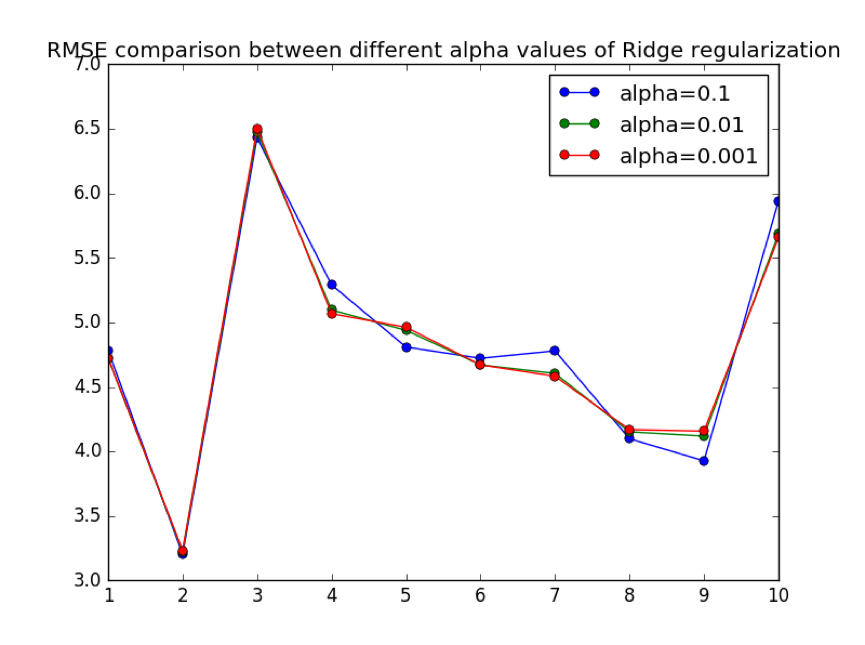
\includegraphics[width=.6\textwidth]{rr.png}
\caption{Ridge Regularization of Boston Dataset}
\label{fig:rr}
\end{figure}
For a clearer comparison of the all RMSE values, we calculate the mean RMSE upon every 10-fold cross validation and we put all of them in Table \ref{tb}.
\begin{table}
\begin{center}
\caption{Compare between Lasso regression and Ridge regression }
\label{tb}
\begin{tabular}{|r|r|r|}
\hline
Value of $\alpha$ & Lasso regularization & Ridge regularization\\
\hline
0.1&5.8639&4.7981\\
0.01&4.9307&4.7686\\
0.001&4.7861&4.7725\\
\hline 	
\end{tabular}
\end{center}
\end{table}
From the above table, we find out that for Lasso regularization, the RMSE is worsened but the sparsity of regression coefficients is obtained. And for Ridge regularization, we get the best RMSE result at α=0.01, which prove that with the control of over fitting, we may get a better model.

\end{document}